\documentclass[10pt,a4paper]{article}
\usepackage{sectsty}
\usepackage{hyperref}
\sectionfont{\raggedright}
% Added to the course template: figures, maths and tables
\usepackage[T1]{fontenc}
\usepackage{graphicx}
\usepackage{amsmath,amssymb}
\usepackage{booktabs}
\usepackage{tabularx}
\usepackage{float}
\usepackage{xurl}
\newcolumntype{Y}{>{\raggedright\arraybackslash}X}
\setlength{\emergencystretch}{2.5em}

\title{Investor Tribes: Hidden Groups of Stocks in SEC Form 13F Filings}
\author{
  Izan Gael Rooke Mora\\
  \texttt{irooke@albertschool.com}%
  \and
  Oussama Maaref\\
  \texttt{omaaref@albertschool.com}%
  \and
  Ryan Ebanda\\
  \texttt{rebanda@albertschool.com}
}
\date{Graph Analytics, Albert School x Mines Paris, November 2026\\[2pt]
Code and data: \url{https://github.com/IzanGael/graph-analytics-13f-coholding}}

\begin{document}
\maketitle

\begin{abstract}
Official sectors group companies by what they do. We ask whether the investors who own stocks group them differently. From the SEC Form~13F holdings of 6,100 to 8,200 US institutional managers over 19 quarters (2021Q4--2026Q2), we build, for each quarter, a graph of the 1,000 largest companies in which two stocks are linked when they share significantly more investors than a bipartite configuration model predicts. Louvain communities in this \emph{ownership graph} are strong (modularity 0.62) and overlap little with Fama--French sectors (NMI 0.13), but partly reflect company size (NMI 0.30). They persist and drift slowly: neither six predefined macro regimes nor a data-driven segmentation finds abrupt reorganisations (permutation $p$-values 0.34 to 0.84). Because a yes/no ownership graph cannot see portfolio rotation, we build a second, \emph{conviction graph} from managers' relative overweights. Its communities differ from ownership groups (ARI 0.29), are not driven by size (NMI 0.13), and read as investor ``tribes'' defined by who bets on them (merger arbitrage, Canadian home bias, income, AI hardware). In a no-look-ahead test, sectors explain next-quarter co-movement better than tribes (8.9\% vs 5.9\% of the cross-section above random groupings), but tribes add 3.8\% on top of sectors and size in 17 of 18 quarters, and do better than sectors in stress quarters.
\end{abstract}

%=====================================================================
\section{Introduction}
Portfolio risk is usually organised by sector: technology, banks, energy. Yet stocks are bought and sold by people, not by sectors. If the same investors hold or bet on the same stocks, those stocks share the same marginal buyers and sellers, and may fall together when those investors reduce risk, whatever their sector. This hidden concentration, often called \emph{crowding}, is invisible in sector labels. Networks are a natural language for such shared exposures \cite{newman2003}.

Our question has three parts:
\begin{itemize}
  \item \textbf{Q1, difference:} do groups of stocks formed by shared investors differ from official sectors?
  \item \textbf{Q2, persistence:} do these groups last over time, and do they reorganise when the macro-economic regime changes?
  \item \textbf{Q3, co-movement:} do they predict which stocks move together next quarter, better than sectors do?
\end{itemize}
\noindent\textbf{Business value.} A map of who owns, and who bets on, the same stocks reveals hidden risk groups that sector labels miss, and tells a portfolio manager whom they will be selling alongside when crowded positions unwind.

The project starts from non-graph data (holdings tables) and builds a justified graph model. Our contributions are: a statistically filtered co-holding network for 19 quarters; tests of whether investor groups follow macro regimes, including a reverse, data-driven ``investor calendar''; a second graph built from allocation weights, whose communities turn out to be investor tribes; and an out-of-sample co-movement test.

%=====================================================================
\section{Dataset Presentation}
\subsection{Source and motivation}
Institutional managers with more than USD 100 million in US equities must file Form~13F with the US Securities and Exchange Commission (SEC) every quarter, listing their long positions at quarter end. The SEC publishes these filings as quarterly structured data sets \cite{sec13f}. We use 19 releases covering the report periods 31~December~2021 to 30~June~2026. The source is official, public and quarterly, and it is naturally bipartite (managers hold stocks), so a graph is natural but not trivial: which stocks ``go together'' has to be derived. Sector labels come from SEC EDGAR files (company CIK and SIC code) \cite{secedgar}, OpenFIGI (CUSIP to ticker and security type) \cite{openfigi}, and the Fama--French 12 and 48 industry definitions \cite{frenchlib}.

\paragraph{Why this dataset.} We chose it after comparing two candidate topics in a small feasibility test (scripts in \texttt{feasibility/}): World Bank contract awards \cite{worldbank} and SEC 13F holdings. The World Bank firm--country graph was poorly suited to our purpose: 95\% of firms worked in a single country, the most central nodes were audit firms rather than meaningful actors, and its communities were unstable between periods (ARI 0.19). The 13F co-holding graph gave interpretable communities that were more stable from one quarter to the next (ARI 0.42 in the same test). 13F also has three practical advantages: it is official, free and released every quarter, so persistence over time can be tested; it covers thousands of managers and nearly every large US company; and the question it answers, hidden crowding risk, matters directly to portfolio managers.

\subsection{Cleaning and universe}
\begin{itemize}
  \item \textbf{Filings:} for each manager and quarter, the latest RESTATEMENT amendment if any, otherwise the original 13F-HR; NEW HOLDINGS amendments add positions.
  \item \textbf{Positions:} long share positions only (options excluded); placeholder CUSIPs removed. Values are corrected for unit errors; filers with implausible values keep their links but not their value.
  \item \textbf{Stocks:} one node per issuer (first six CUSIP characters, which merges share classes).
  \item \textbf{Universe per quarter:} the 1,000 largest operating companies by reported value (funds and ETFs excluded) held by at least 50 managers. They hold about 92\% of reported value; sector coverage is 96.3\% (2021Q4) to 99.3\% (2026Q2).
\end{itemize}
Per quarter this leaves 731,000 to 1,078,000 manager--stock positions among 6,119 to 8,226 managers.

\subsection{Graph model 1: the ownership graph}
For each quarter we first build a bipartite graph: manager nodes, stock nodes, and an edge when manager $m$ holds stock $i$. We then project it onto stocks. Raw shared-holder counts $C_{ij}$ are dominated by popularity (almost every manager holds Apple, which would be linked to everything), so each count is compared with a chance model.

\paragraph{Chance model.} We use the bipartite configuration model \cite{saracco2015,saracco2017}. Each manager--stock pair gets a probability
\begin{equation}
  p_{im} = \frac{x_i\, y_m}{1 + x_i\, y_m},
  \qquad \text{with } \sum_m p_{im} = k_i \text{ and } \sum_i p_{im} = n_m ,
\end{equation}
so that on average every stock keeps its real number of holders $k_i$ and every manager its real number of positions $n_m$. The expected number of shared holders, its variance and the edge score are
\begin{equation}
  E_{ij} = \sum_m p_{im}\,p_{jm}, \qquad
  V_{ij} = \sum_m p_{im}\,p_{jm}\,\bigl(1 - p_{im}\,p_{jm}\bigr), \qquad
  z_{ij} = \frac{C_{ij} - E_{ij}}{\sqrt{V_{ij}}} .
\end{equation}

\paragraph{Backbone.} A global threshold either keeps a hairball ($z>3$ keeps about 86,500 edges) or isolates most stocks ($z>10$ isolates 767), so each stock keeps its 15 strongest partners with $z>3$ (sensitivity: 10 and 25); an edge exists if either endpoint selects it.

\paragraph{Graph type.} Nodes are stocks; an edge means ``significantly more shared holders than chance''; the weight is $z_{ij}$, and $C_{ij}$ is kept as an attribute. The graph is \emph{undirected} because co-holding is symmetric, and \emph{simple} because we build one graph per quarter instead of a multigraph across quarters; time is handled by comparing quarters.

\subsection{Graph model 2: the conviction graph}
The ownership graph only records whether a manager holds a stock. Managers rarely sell a position completely; they trim and add. A fund going from 40\% to 5\% in Nvidia and from 5\% to 60\% in Exxon looks unchanged in a yes/no graph. We therefore build a second graph from allocation weights. With $w_{ms}$ the weight of stock $s$ in manager $m$'s portfolio, $W_s$ the stock's share of all reliable 13F value in the universe, and $S_m$ the set of stocks held by $m$, the \emph{relative overweight} is
\begin{equation}
  \mathrm{OW}_{ms} \;=\; \frac{w_{ms}}{W_s \big/ \sum_{s' \in S_m} W_{s'}} ,
\end{equation}
the real weight divided by the weight the stock would have if the manager held its own stocks in market proportions. This separates \emph{which} stocks a manager holds from \emph{how much} of each, in the spirit of active weights \cite{cremers2009}; a plain ratio $w_{ms}/W_s$ would label almost every position of a small fund as a bet. A \emph{bet} is $\mathrm{OW}_{ms}>2$ (sensitivity: 1.5 and 3); managers need at least 10 positions and flagged filers are excluded. About 22\% of positions are bets (155,000 to 234,000 per quarter, from 4,900 to 6,900 managers), and mega-caps are rarely bets (1\% to 6\% of their holders). The manager--bet graph is projected exactly like the ownership graph (same chance model, top 15, $z>3$).

\subsection{Graph statistics}
Table~\ref{tab:graph} reports the size, connectivity and distance measures of both graphs.

\begin{table}[H]
\centering\footnotesize\setlength{\tabcolsep}{3pt}
\caption{Graph statistics. Distances are computed on the largest connected component (LCC), in hops.}
\label{tab:graph}
\begin{tabularx}{\linewidth}{@{}p{2.8cm}p{2.05cm}p{2.05cm}Y@{}}
\toprule
Measure & Ownership 2026Q2 & Conviction 2026Q2 & 19 quarters (own. / conv.) \\
\midrule
Nodes / edges & 1,000 / 10,134 & 1,000 / 10,327 & edges 9,541--10,134 / 9,791--10,384 \\
Mean degree / density & 20.3 / 0.020 & 20.7 / 0.021 & 19.1--20.3 / 19.6--20.8 \\
Components (isolated) & 54 (47) & 17 (14) & 54--86 / 7--18 \\
Largest component & 934 & 982 & 907--940 / 982--994 \\
Diameter / radius & 14 / 7 & 8 / 5 & 11--18, 6--9 / 8--10, 5 \\
Average shortest path & 3.58 & 3.10 & 3.47--3.80 / 3.09--3.16 \\
Average clustering & 0.35 & 0.29 & 0.31--0.35 / 0.24--0.29 \\
Louvain groups / modularity & 16 / 0.62 & 12 / 0.58 & mod.\ 0.62--0.64 / 0.54--0.60 \\
\bottomrule
\end{tabularx}
\end{table}

%=====================================================================
\section{Description of the Analysis}
\subsection{Connectivity, distances and centralities}
Components are counted on all 1,000 stocks; a stock is isolated when none of its 15 best partners passes $z>3$. Because both graphs are disconnected, diameter and radius are computed on the largest connected component (91\% to 99\% of stocks), in hops: $z$ is a similarity, not a distance, so it is not used as an edge length. We compute degree, strength (sum of $z$), betweenness, closeness, eigenvector centrality (weighted by $z$), PageRank (weighted, damping 0.85), the $k$-core number, and a bridge score, the participation coefficient
\begin{equation}
  P_i = 1 - \sum_{c} \left(\frac{k_{ic}}{k_i}\right)^{2},
\end{equation}
where $k_{ic}$ is the number of links from stock $i$ into community $c$ ($P_i=0$ when all links stay inside its own community).

\subsection{Communities}
We use Louvain modularity optimisation \cite{blondel2008,newman2006} with weight $z$, run 20 times per quarter (seeds 42 to 61), and keep the run with the highest modularity. Agreement between two groupings is measured by the adjusted Rand index (ARI; 1 = identical, 0 = chance level) \cite{hubert1985} and normalised mutual information (NMI) \cite{strehl2002}. Group labels are arbitrary, so quarters are always compared by membership, never by label.

\subsection{Macro regimes and the investor calendar}
The team defined six regimes from inflation, growth, real rates, volatility and the dominant market driver: Repricing (2021Q4--2022Q3), Disinflation (2022Q4--2023Q2), AI soft landing (2023Q3--2024Q4), Tariff shock (2025Q1--Q2), Boom with a soft labour market (2025Q3--Q4) and Energy shock (2026Q1--Q2). They give 5 boundaries among the 18 quarter-to-quarter transitions. We test whether links or communities change more at boundaries; significance comes from exact permutation tests over all $\binom{18}{5}=8{,}568$ placements of 5 boundaries. In reverse, an \emph{investor calendar} cuts the 19 quarters into consecutive blocks by dynamic programming (cost = within-block dissimilarity) and compares the result with a smooth-drift null that keeps the mean similarity at each time gap and shuffles the residuals. Break strength at a transition is the mean similarity within a two-quarter window on each side minus the mean similarity across it.

\subsection{Co-movement}
Quarterly price returns are computed from the filings themselves: the median of value/shares across reliable filers, corrected for stock splits (checked on Nvidia, Amazon and Alphabet; dividends are not included). For each of the 18 periods, groups known at quarter $t$ explain returns from $t$ to $t+1$ (no look-ahead). With $r_i$ the return of stock $i$ and $\bar r_{g}$ the mean return of its group,
\begin{equation}
  R^2 = \frac{\sum_i \left(\bar r_{g(i)} - \bar r\right)^2}{\sum_i \left(r_i - \bar r\right)^2},
  \qquad
  \Delta R^2 = R^2 - \overline{R^2}_{\text{random}},
\end{equation}
where the random term averages 200 groupings with the same group sizes (more groups always explain more by chance). We also measure the incremental $R^2$ of tribes on top of Fama--French~12 sectors and size quintiles (OLS with group dummies).

\subsection{Software, parameters, code reuse and AI use}
The analysis uses Python 3.11--3.14, NetworkX 3.6 \cite{hagberg2008} (graphs, Louvain, centralities), pandas, NumPy, SciPy and scikit-learn (ARI, NMI). Neo4j 5.26 \cite{neo4j} was used only to visualise the tribes for the oral defense. All parameters are set in \texttt{src/config.py} and \texttt{src/regimes/}; the repository README \cite{repo} gives the run order and the link to the processed data, which is too large for GitHub.

\paragraph{Code reuse.} No existing code for these data sets was copied from the internet or from other projects; all scripts were written for this project. Methods from the literature are cited.

\paragraph{AI use.} We used Claude Code \cite{claudecode} throughout: to summarise the course instructions, write and run the data pipeline, the graph construction, the regime, conviction and co-movement scripts and the Neo4j demo, review code, explain methods and draft text, including this report. The students made every analytical decision (topic, quarters, filters, chance model, backbone, adding regimes, the move to allocations, the overweight rule and threshold, the tribe names) and checked the results; failures and results against our hypotheses are reported as such. A detailed log is in \texttt{docs/AI\_USE.md}.

%=====================================================================
\section{Results}
\subsection{Connectivity and distances}
Neither graph is connected (Table~\ref{tab:graph}), so distances are reported on the largest component. The conviction graph is more connected and more compact: any two stocks are about three steps apart, against 3.6 in the ownership graph, and its diameter is 8 against 14. Bets connect the market more tightly than plain ownership.

\subsection{Centralities}
\begin{table}[H]
\centering\footnotesize\setlength{\tabcolsep}{3pt}
\caption{Most central stocks, 2026Q2 (largest component).}
\label{tab:central}
\begin{tabularx}{\linewidth}{@{}p{2.4cm}YY@{}}
\toprule
Centrality & Ownership graph & Conviction graph \\
\midrule
Degree / PageRank & Voya, Dollar Tree, Synchrony, Reinsurance Group, MetLife & Five Below, Viavi, Axis Capital, Dynatrace, Reinsurance Group \\
Betweenness & Newmont, Voya, Burlington, Hartford, Synchrony & Five Below, Viavi, Axis Capital, Dynatrace, Ingram Micro \\
Eigenvector & Merck, Procter \& Gamble, Coca-Cola, PepsiCo, Home Depot & Fortis, Emera, Scotiabank, TD, Rogers (Canadian tribe) \\
Bridge score & Annaly, Southwest, Newmont, Delta, Targa & T-Mobile, Ingersoll Rand, Ferguson, West Pharma, Annaly \\
Spearman with size (eig.\ / degree) & $+0.77$ / $+0.15$ & $-0.52$ / $-0.60$ \\
Innermost $k$-core & 769 stocks, all groups & 31 stocks, all Canadian tribe \\
\bottomrule
\end{tabularx}
\end{table}
In the ownership graph, eigenvector centrality is almost a popularity measure (Spearman 0.90 with the number of holders): its top stocks are the consensus blue chips. Degree and PageRank are nearly uncorrelated with popularity (0.17 and 0.12), as intended by the chance model and the top-15 rule, and pick mid-caps that many crowds share. In the conviction graph the picture flips: centralities fall with company size (Spearman $-0.5$ to $-0.7$). Active bets concentrate on small and mid caps, while mega-caps, held by everyone but bet on by almost no one, sit on the periphery. The highest bridge scores (T-Mobile, Ingersoll Rand, Ferguson, NXP, Cheniere) identify stocks bet on by several tribes: potential contagion points if one tribe sells.

\subsection{Ownership communities versus sectors (Q1)}
Louvain finds about 15 ownership groups per quarter (modularity 0.62--0.64), and two runs on the same quarter agree at ARI 0.79, so the structure is robust. Overlap with Fama--French~12 sectors is low in every quarter (NMI 0.12--0.15), but overlap with size quintiles is higher (NMI 0.30): managers specialise by market capitalisation, so part of ``different from sectors'' is ``large stocks together''. This size confound motivates the conviction graph.

\subsection{Persistence and macro regimes (Q2)}
\begin{figure}[H]
\centering
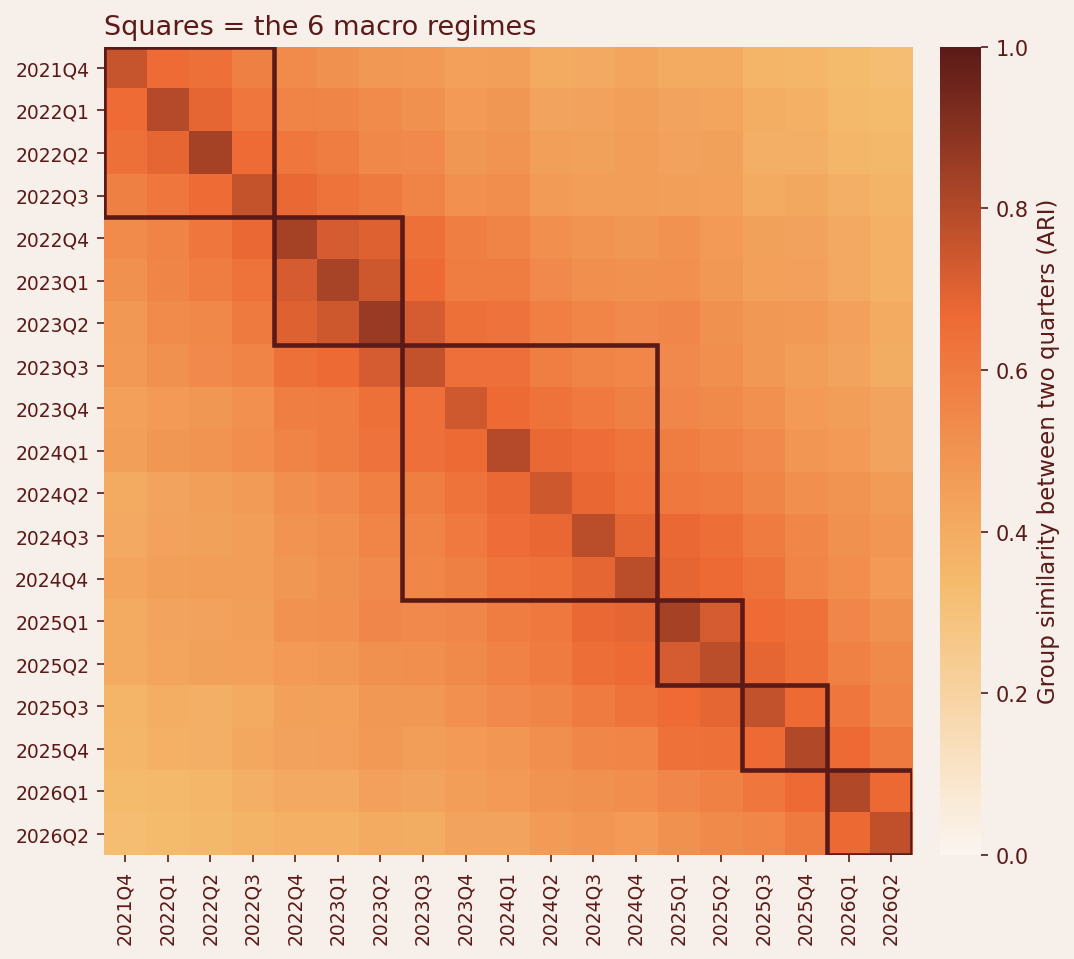
\includegraphics[width=0.62\linewidth]{figures/f2_regime_heatmap.png}
\caption{Similarity (ARI) of ownership communities between every pair of quarters; squares are the six macro regimes. Similarity fades smoothly with time, with no darker blocks inside regimes.}
\label{fig:regimes}
\end{figure}

\begin{table}[H]
\centering\footnotesize\setlength{\tabcolsep}{3pt}
\caption{Regime tests on the ownership graph (exact permutation tests; 5 boundaries vs 13 other transitions).}
\label{tab:regimes}
\begin{tabularx}{\linewidth}{@{}Ylll@{}}
\toprule
Test & Inside & Boundary & $p$ \\
\midrule
A. Link overlap of consecutive quarters (Jaccard) & 0.491 & 0.493 & 0.61 \\
B. Community overlap of consecutive quarters (ARI, best run) & 0.744 & 0.771 & 0.84 \\
B$'$. Same, averaged over $20\times20$ Louvain runs & 0.682 & 0.687 & 0.65 \\
C. Same vs different regime at equal time gap (1--5 quarters) & & & 0.68 \\
D. Investor calendar (3--6 blocks) vs smooth drift & & & $\geq 0.34$ \\
E. Break strength, macro boundaries vs others & 0.039 & 0.048 & 0.11 \\
\bottomrule
\end{tabularx}
\end{table}
Ownership communities persist: about two thirds of links reappear the next quarter, and community similarity falls slowly from 0.68 after one quarter to 0.57 after one year and 0.33 after four and a half years (Figure~\ref{fig:regimes}). None of the tests finds a regime effect (Table~\ref{tab:regimes}). The best data-driven cuts explain no more than cuts of a smooth drift, so investors do not have regimes of their own either. The sharpest changes occur into 2022Q3 and 2022Q4 (the 2022 rate shock) and into 2026Q1 (the energy shock), while the short 2025 tariff panic is an ordinary quarter; macro boundaries are slightly sharper on average, but not significantly ($p=0.11$).

\subsection{The conviction graph: investor tribes}
\begin{figure}[H]
\centering
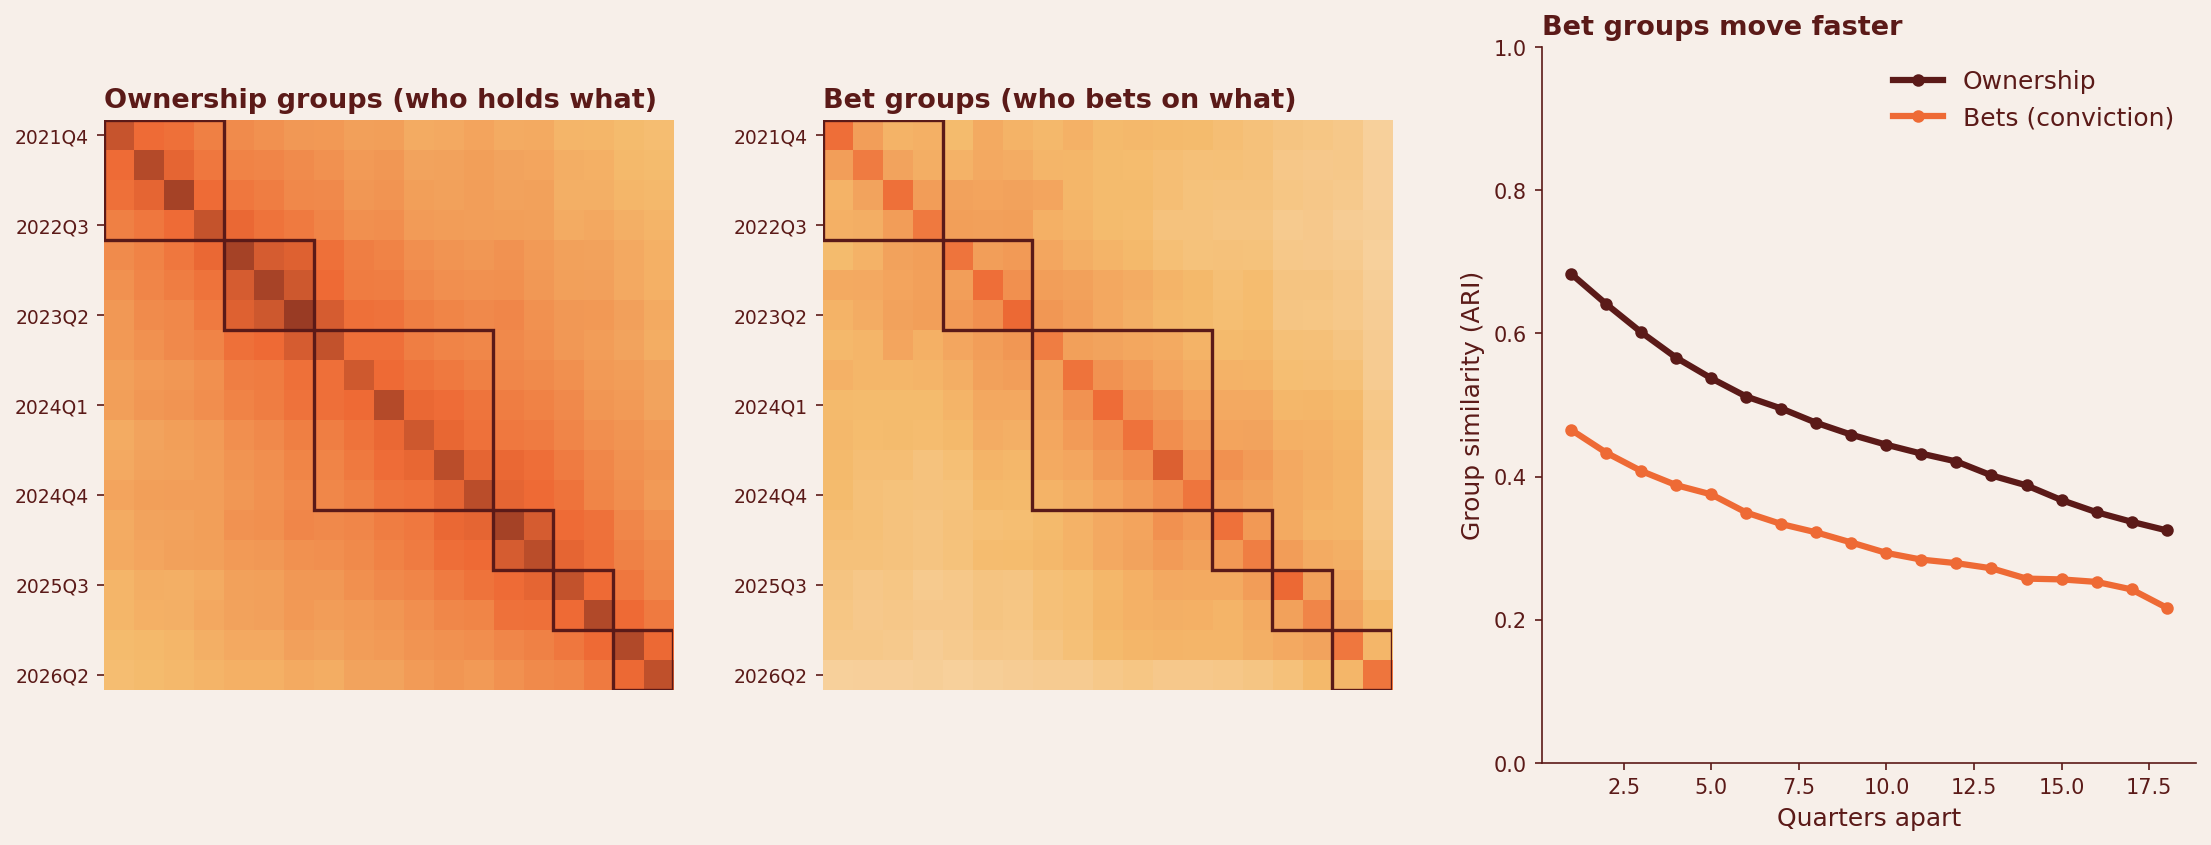
\includegraphics[width=\linewidth]{figures/f4_ownership_vs_conviction.png}
\caption{Community similarity between quarters for ownership groups (left) and bet groups (middle), and mean similarity by time gap (right).}
\label{fig:conviction}
\end{figure}
Bet groups are a different map from ownership groups (ARI 0.29 in the same quarter), are not a size effect (NMI with size 0.13 against 0.30), and overlap sectors as little as ownership groups (0.14). They change faster (Figure~\ref{fig:conviction}): similarity 0.47 after one quarter and 0.22 after four and a half years, against a run-to-run noise level of 0.63 (0.79 for ownership), so the change exceeds the algorithm's noise. Yet they show no regime effect either (consecutive quarters $p=0.34$, equal gap $p=0.46$; thresholds 1.5 and 3 give 0.24--0.78, with one borderline 0.07 that the other tests do not confirm).

Profiling the bet groups of 2022Q2 and 2026Q2 (key stocks, sector and size mix, and the managers with most bets in each group) shows that they are defined by \emph{who} bets on them: investor tribes (Table~\ref{tab:tribes}). The clearest case is merger arbitrage. In 2022Q2 one group contains Activision, VMware, Twitter, Citrix and Zendesk, all pending takeover targets, bet on by Gabelli, Millennium, Verition, Pentwater and Prelude; in 2026Q2 a group of new deal targets (Warner Bros Discovery, Electronic Arts, Chart Industries) is again bet on by Gabelli, Prelude and Verition. The graph finds this theme without any information on mergers.

\begin{table}[H]
\centering\footnotesize\setlength{\tabcolsep}{3pt}
\caption{Bet groups of 2022Q2 and 2026Q2 (names chosen by the team from the evidence; Jaccard overlap of members in brackets).}
\label{tab:tribes}
\begin{tabularx}{\linewidth}{@{}p{2.5cm}YYp{2.1cm}@{}}
\toprule
Tribe & Key stocks & Main bettors & 2022Q2 $\to$ 2026Q2 \\
\midrule
Canadian home bias & TD, RBC, BMO, BCE, Fortis & Canadian banks' asset managers & stable (0.60) \\
Rate-sensitive income & Apartment REITs, utilities & Pension funds, insurers & merge (0.46) \\
Blue-chip dividend & PepsiCo, Verizon, P\&G, J\&J & Trust co., wealth managers & grows (0.38) \\
International ADRs & China tech $\to$ EU/JP banks & Global quant, wealth & rotates (0.40) \\
Merger arbitrage & Pending takeover targets & Gabelli, Prelude, Verition & same funds, new deals \\
2021 growth casualties & RingCentral, Teladoc, Zscaler, Snap & Multi-strategy hedge funds & dissolves \\
AI hardware + biotech & Viavi, Semtech, FormFactor, Micron, AMD & Millennium, Jump, Algert & new in 2026 \\
Midstream + private mkts & Energy Transfer, Williams, KKR, Apollo & Infrastructure/MLP specialists & new in 2026 \\
\bottomrule
\end{tabularx}
\end{table}

\subsection{Co-movement (Q3)}
\begin{figure}[H]
\centering
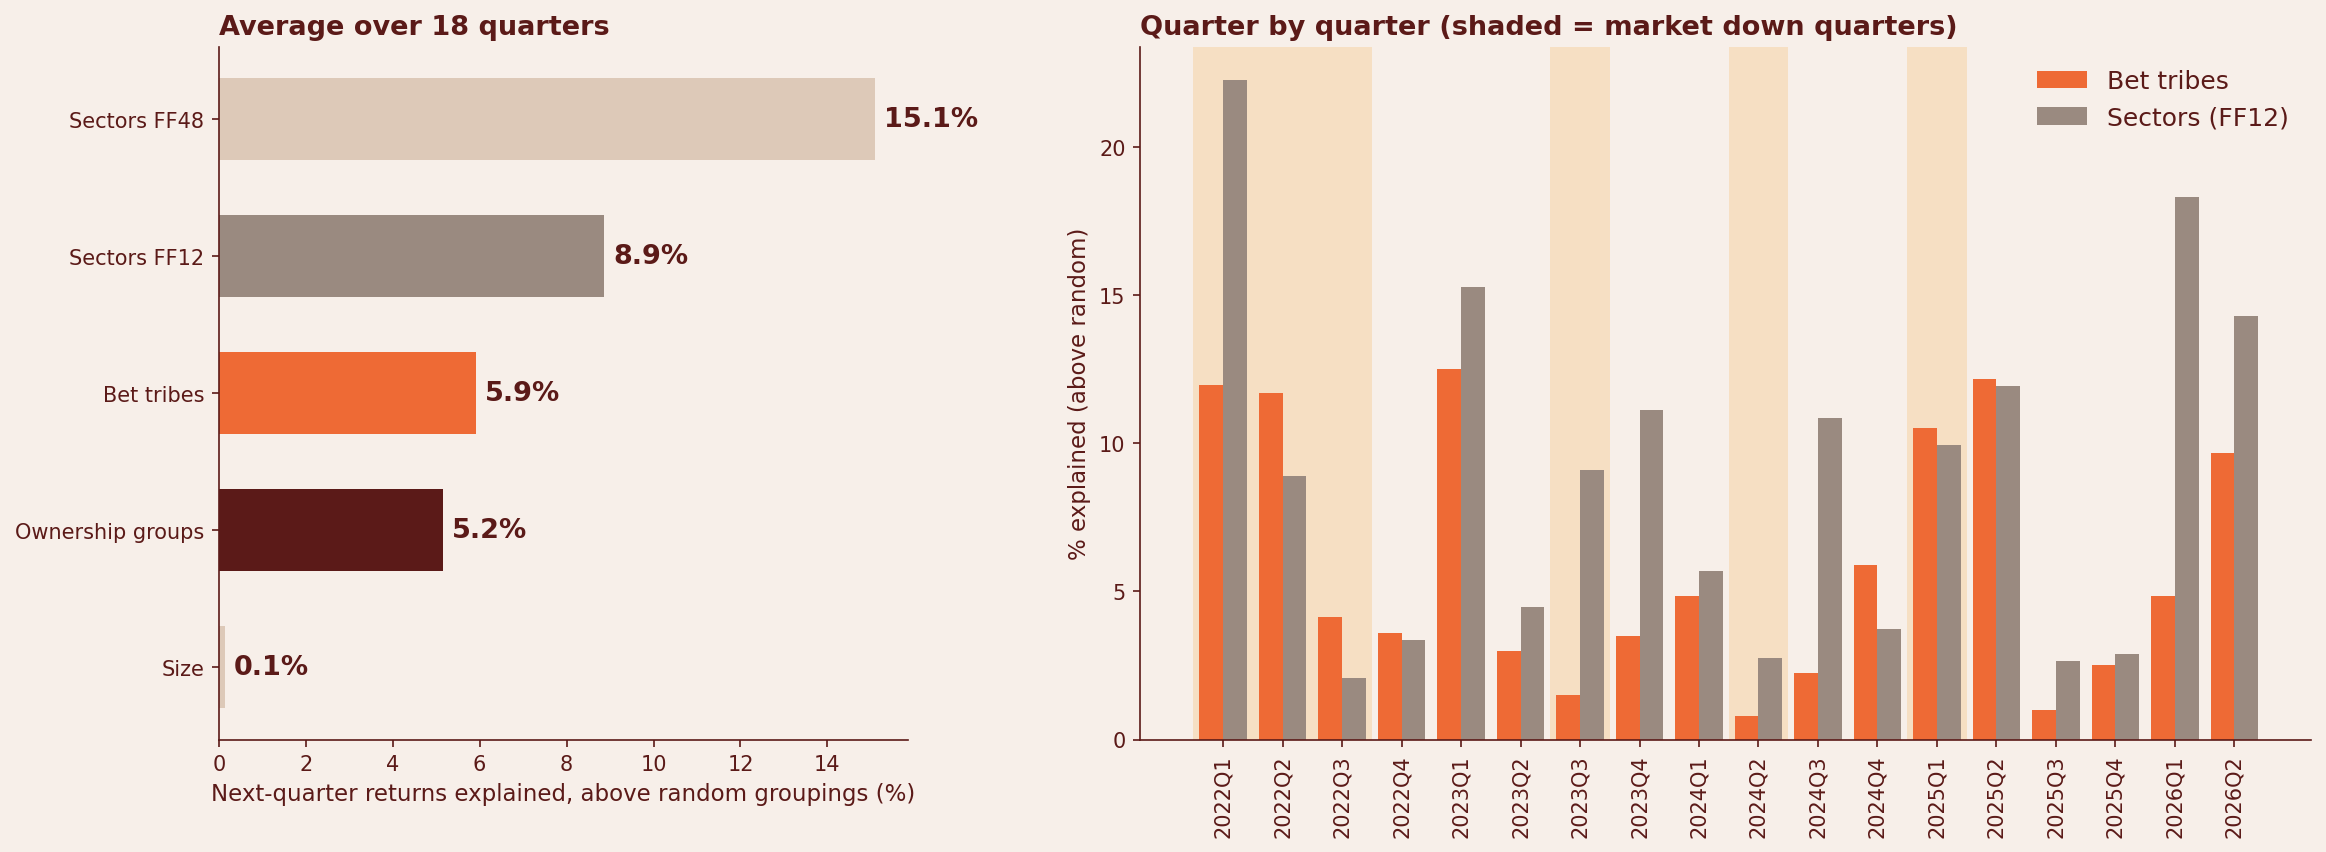
\includegraphics[width=\linewidth]{figures/f6_comovement.png}
\caption{Share of next-quarter returns explained by each grouping, above random groupings of the same sizes: mean over 18 periods (left) and by period for tribes and FF12 sectors (right; shaded = market down quarters).}
\label{fig:comove}
\end{figure}

\begin{table}[H]
\centering\footnotesize\setlength{\tabcolsep}{4pt}
\caption{Co-movement test: groups at $t$, returns from $t$ to $t+1$ (18 periods, 6 down quarters). Values are $\Delta R^2$.}
\label{tab:comove}
\begin{tabular}{@{}lcccc@{}}
\toprule
Grouping (avg.\ groups) & Mean & Down quarters & Up quarters & Periods $p<0.05$ \\
\midrule
Bet tribes (9.7) & 5.9\% & 6.8\% & 5.5\% & 18 / 18 \\
Ownership groups (10.7) & 5.2\% & 5.2\% & 5.1\% & 16 / 18 \\
Fama--French 12 sectors & 8.9\% & 9.2\% & 8.7\% & 18 / 18 \\
Fama--French 48 sectors & 15.1\% & 14.8\% & 15.2\% & 18 / 18 \\
Size quintiles & 0.1\% & 0.5\% & 0.0\% & 2 / 18 \\
\bottomrule
\end{tabular}
\end{table}
Sectors explain co-movement better than tribes (Table~\ref{tab:comove}): the hypothesis ``better than sectors'' is not supported. But tribes carry information that sectors do not: on top of FF12 sectors and size quintiles they add 3.8\% of explained variance (above random), significant in 17 of 18 periods (ownership groups add 3.4\%, 15 of 18). Tribes beat ownership groups in 11 of 18 periods, especially in down quarters (6.8\% vs 5.2\%), and beat FF12 sectors in the 2022 crash (2022Q2--Q3) and around the 2025 tariff shock (2025Q1--Q2) (Figure~\ref{fig:comove}): when markets are stressed, who bets on a stock matters relatively more. These are associations, not causal effects.

%=====================================================================
\section{Conclusions}
\begin{itemize}
  \item \textbf{Q1.} Investor groups differ from sectors. Ownership groups are partly size classes; conviction groups are not, and read as investor tribes defined by who bets on them.
  \item \textbf{Q2.} Groups persist and drift slowly. They do not reorganise at macro regime boundaries, and investors have no data-driven regimes of their own; only deep, lasting shocks (2022, 2026) coincide with the fastest change, as a hint rather than a proof. Bet groups rotate faster than ownership groups, following deals and themes rather than the macro calendar.
  \item \textbf{Q3.} Sectors remain the best single predictor of co-movement, but tribes are a significant complementary layer, most useful in stress quarters.
\end{itemize}
\noindent\textbf{Business value.} Sectors are the first risk map; investor tribes are a hidden second layer. A portfolio manager can see which tribe shares their positions (owning Warner Bros in 2026 means sitting next to the merger-arbitrage funds), refresh the map about once a year because it drifts slowly, and watch tribe-level crowding most closely in stressed markets.

\noindent\textbf{Limitations.} Form~13F covers long US equity positions of large managers only, at quarter end, with up to 45 days' delay, and a filer is an institution, not a single fund. Value-cleaning thresholds were not tuned. Regime dates are approximate and should be sourced (for example from FRED series), and with 19 quarters and 5 boundaries the regime tests have limited power. Returns are price returns built from the filings. Tribe names are interpretations, and Louvain results vary slightly with seeds and library versions.

\noindent\textbf{Future work.} Track each tribe over all 19 quarters to date when themes form; test whether tribe-level selling (from changes in shares held) predicts falls; compare Louvain with label propagation; and run the remaining sensitivity checks (top 500 and 2,000 stocks, alternative co-holding weights).

\bibliographystyle{plain}
\bibliography{biblio}

\end{document}
